\documentclass{article}


\usepackage{graphicx} % Required for inserting images
\usepackage{graphicx} % Required for inserting images
\usepackage{graphicx} % Required for inserting images
\usepackage{amsmath}
\usepackage{amsfonts}
\usepackage{amssymb}
\usepackage{graphicx}
\usepackage{subfigure}
\usepackage{booktabs}
\usepackage{ctex} % Need for inserting Chinese characters, also needed to change compiler from pdfLaTex to XuLaTex

\usepackage[usenames,dvipsnames]{xcolor}
\usepackage{fancybox}
\usepackage{tikz}
\usetikzlibrary{arrows,snakes,backgrounds}
\usepackage{hyperref}

\tikzstyle{place}=[circle,draw=blue!50,fill=blue!20,thick]
\pagestyle{plain} 
%%%%%%%%%% EXACT 1in MARGINS %%%%%%% 

\textheight235truemm\textwidth165truemm
\voffset-2.2cm\hoffset-1.2cm \vfuzz=10000truept\hfuzz=10000truept
\usepackage{lipsum}
\usepackage[usestackEOL]{stackengine}[2013-10-15]
\def\x{\hspace{1.5ex}}
\def\y{\hspace{1.225ex}}
\def\z{\hspace{1.9ex}}
\newcommand{\RED}[1]{{\color{red}{#1}}}
\newcommand{\ignore}[1]{}
\newcommand{\Matrix}[1]{\ensuremath{\left(\begin{array}{rrrrrrrrrrrrrrrrrr} #1 \end{array}\right)}}
\newcommand{\Matrixc}[1]{\ensuremath{\left(\begin{array}{cccccccccccc} #1 \end{array}\right)}}
\newcommand{\Matrixs}[1]{\ensuremath{\left[\begin{array}{cccccccccccc} #1 \end{array}\right]}}
\newcommand{\etal}{{\it et al.}}
\newcommand{\multiple}{{multiple} }

%\newcommand{\Kcomment}[1]{{\color{blue}{[KJ: #1]}}}

%\newcommand{\RED}[1]{{\color{red}{#1}}}

\newcommand{\GG}{{\mathcal{G}}}
\newcommand{\R}{{\mathbb{R}}}
\newcommand{\Z}{{\mathbb{Z}}}
\newtheorem{theorem}{Theorem}[section]
\newtheorem{lemma}[theorem]{Lemma}
\newtheorem{definition}[theorem]{Definition}
\newtheorem{corollary}[theorem]{Corollary}
\newtheorem{proposition}[theorem]{Proposition}
\newtheorem{remark}[theorem]{Remark}
\newtheorem{remarks}[theorem]{Remarks}
\newtheorem{example}[theorem]{Example}
\newtheorem{claim}[theorem]{Claim}


\usepackage[
backend=biber,
style=alphabetic,
sorting=ynt
]{biblatex}
\addbibresource{Chinese_med.bib, network.bib}

\title{Local and Global Motifs in Traditional Chinese Medicine}
\author{Carter Feng and Yunjiao Wang}
%\date{}


\begin{document}

\maketitle
\begin{abstract}
    Traditional Chinese Medicine is powerful and attractive alternative medicine in the West. Its holistic approach could complement modern western medicine and also could provide guideline to design multi-target treatment strategy. Moreover, TCM is accessible to average people, which could    
\end{abstract}
\section{Introduction}
Traditional Chinese medicine (TCM) has been widely recognized  and becomes an invaluable component in alternative medicines in the west \cite{Kaptchuk2000} though it is not always viewed correctly.   Chinese medicine is the result of science over long time as it is the result of continuous critical thinking and extensive clinical observations and testing \cite{Kaptchuk2000}. It is a coherent and independent system of thoughts and practice that have been developed over 2000 years.   As Manfred Porkert \cite{Porkert1990} rightly pointed out, Chinese medicine is not less logical than the Western, just less analytical. In this project, we aim to contribute analytical study of Chinese medicine. 

TCM is an attractive alternative for several reasons.
First, TCM takes holistic approach, which takes into account of not only interactions among different components within the whole body, but also external environment such as season, time of the day, the place of living and so on. This approach is very different from that of modern medicine, which essentially treat a patient as an independent sick organ with a bunch of testing numbers. It is so often that disease spread from one organ to another. TCM has the principle that strengthen the still healthy organ that is directly impact by the ill organ before treat the sick one so to prevent spread. This can only be achieved by knowing the overall relations between the organs. Second, because of holistic approach, TCM natually uses multi-target approach instead of single-target as  modern medicine usually does (add citation). This approach could provide a balanced and effective treatment with less side effect. Third, TCM focuses on health, not disease. For example, it is so common that we feel something is going wrong, for example feeling lack of energy, but all medical tests show nothing wrong. INSERT A PICTURE OF DIFFERENCE BETWEEN SICK AND UNHEALTHY. TCM is able to detect root problems by examining your complexion, tong, pulse and other factors. According to Huang Di Nei JIng, the best doctor is the one who  bring patient back to true healthy before the patient even gets sick. 
Finally,  TCM  is very  accessible to average people. In the past, Chinese has some general idea on diagonizing and even able to construct some treatments by themselves for minor problems, though not always work.  The parents and grant parents (none of them are medical professionals, but with general knowledge of herbs) of the second author had successfully treat themselves for problem
such as inflammation of the sinuses (a single-time wash of sinuses using the flower of Hibiscus mutabilis cured the chronic problem the author had for several years), red eye， high blood pressure, blue nose,  fatigue and so on.  The grant parents never saw a modern doctor and lived for about 90 years.  

Imagine that if everybody can identify themselves health issue before gets sick, then the immense cost in medical can be saved,  the pollution related to drugs can be dramatically reduced, and  people can live healthier and longer and happier.

TCM is developed based on theories and principles described in the ancient work Huang Di Nei Jing. The main theories are based on two networks: a five-node network called five-element system, and a two-node network called yin-yang relation.  Diagonsis and treatments are conducted based on the dynamics of the two networks.  In this work, we aims to introduce and understand the theories from network dynamics point of view. 


Network motif was proposed to understand dynamics of complex network systems by looking at small sub-networks that occur more often than usual or functionally building blocks \cite{milo2002, Alon2007}. It is  known that the dynamics of a sub-network  in general may not reflect the dynamics of the whole system. However, if the  sub-network is relatively independent, then its dynamics can be manifested in the dynamics of the whole system.  For example, the sub-network is an isolated network, or it does not have input from remaining networks. 

In TCM, the principles in diagnosis and treatments are based on the sub-networks  of the five-element network.
This indicates the activity at a local sub-network can be roughly isolated at short term. That is, TCM assumes implicitly the existence of different time scales. This assumption is reasonable as we all know that it takes time for a disease spread from one organ to another even with directed connection. 



The structure of the paper is as follows. ....

\section{Network motifs and principles in TCM}

Five-element diagram (Wu Xing Diagram) is the diagram that is a global motif to describe the interactions among different organs (or organ blocks).  
\begin{figure}[!htb]
\centering
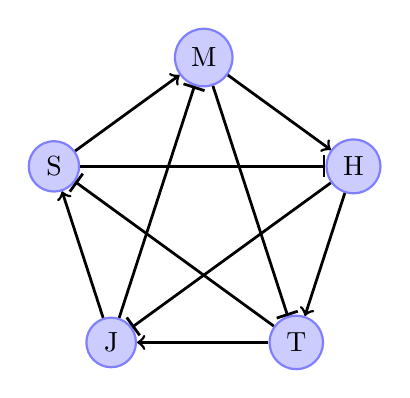
\begin{tikzpicture}[line width=1pt,  scale = 2]
\node[place] (M) at (90:1) {M};
\node[place]  (H) at (18:1) {H};
\node[place]  (J) at (234:1) {J};
\node[place]  (T) at (-54:1) {T};
\node[place]  (S) at ( 162:1) {S};

\path[->] (M) edge (H)
        (H) edge (T)
            (T) edge  (J)
            (J) edge (S)
              (S) edge(M)
        (M) edge[-|] (T)
        (H) edge[-|] (J)
        (T) edge[-|]  (S)
        (J) edge[-|] (M)
        (S) edge[-|] (H);     
 \end{tikzpicture}

\caption{Five-element network}
\label{F:WuXing}
\end{figure}

\begin{figure}[!htb]
\centering
\begin{minipage}{0.2\textwidth}
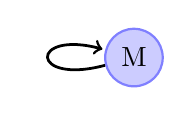
\begin{tikzpicture}[line width=1pt,  scale = 2]
\node[place] (M) at (0:0) {M};

\path[->] (M) edge[loop left] (M);     
 \end{tikzpicture}
 \end{minipage}
 \begin{minipage}{0.2\textwidth}
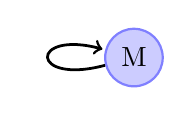
\begin{tikzpicture}[line width=1pt,  scale = 2]
\node[place] (M) at (0:0) {M};

\path[-|] (M) edge[loop left, -|] (M);     
 \end{tikzpicture}
 \end{minipage}
 \begin{minipage}{0.3\textwidth}
 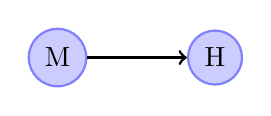
\begin{tikzpicture}[line width=1pt,  scale = 2]
\node[place] (M) at (0:0) {M};
\node[place] (H) at (0:1) {H};

\path[->] (M) edge (H);  
 \end{tikzpicture}
\end{minipage}
 \begin{minipage}{0.3\textwidth}
 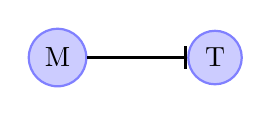
\begin{tikzpicture}[line width=1pt,  scale = 2]
\node[place] (M) at (0:0) {M};
\node[place] (T) at (0:1) {T};

\path[-|] (M) edge (T);  
 \end{tikzpicture}
\end{minipage}
\caption{Examples of One and two-node Motifs. (Left) Self regulation; (Middle) Generation; (Right) Restrain}
\label{F:Motifs}
\end{figure}


\begin{figure}[!htb]
\centering
 \begin{minipage}{0.3\textwidth}
 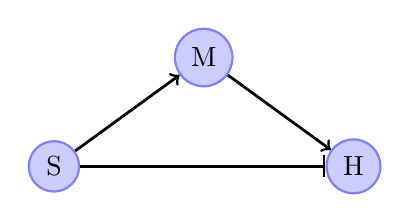
\begin{tikzpicture}[line width=1pt,  scale = 2]
 \node[place] (M) at (90:1) {M};
 \node[place] (S) at (162:1) {S};
\node[place] (H) at (18:1) {H};

\path[->] (M) edge (H)
           (S) edge (M)
        (S) edge[-|](H); 
 \end{tikzpicture}
\end{minipage}
 \begin{minipage}{0.3\textwidth}
 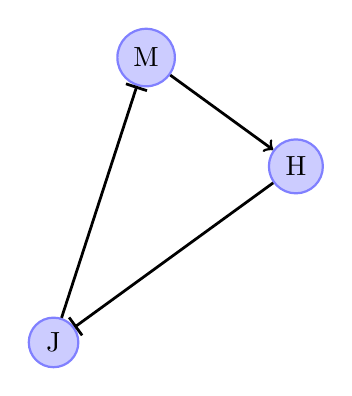
\begin{tikzpicture}[line width=1pt,  scale = 2]
\node[place] (M) at (90:1) {M};
\node[place] (H) at (18:1) {H};
\node[place] (J) at (234:1) {J};

\path[->] (M) edge (H)
(H) edge[-|] (J)
(J) edge[-|] (M);  
 \end{tikzpicture}
\end{minipage}
\caption{three-node Motifs. (Left) Here S (water) is the mother component of M (wood). Strengthen S could make  to M 虚。 }
\label{F:Motifs}
\end{figure}


Two categories of health issues, Excess(实) and  Deficiency (虚). Excess occurs when both pathological energy and   vital normal energy are  strong. It is related to excessive activity (fever), stagnation (Blood stasis), existence of tumor and so on. 
Deficiency arises when vital normal energy is low. It is related to lack of resources. 

Four major principles described next provide general guidance on how to fix Excess and Deficiency.  

\begin{enumerate}
    \item (实则泻其子) If the mother is in  Excess, then reduce  its child element. 
    \item (虚则补其母) If the child is in Deficiency, then strengthen its mother.
    \item (母能令子虚) A mother organ can lead  its child organ towards Deficiency. \cite{nanJing} 
    \item (子能令母实) A child organ can lead its mother organ Excess. 
\cite{nanJing}
    
\end{enumerate}


\section{Dynamics of network motifs}


\subsection{Single-node motif}
Let node $x$ be a component in the five-element network. 
Assume that all other components in the network are normal and are not effect by the activity of the node. 
\begin{figure}[!htb]
\centering
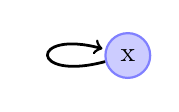
\begin{tikzpicture}[line width=1pt,  scale = 2]
\node[place] (x) at (0:0) {x};
%\node[] (M) at (0:-1) {M};
%\node[] (C) at (210:1) {C};

\path[->] (x) edge[loop left] (x);
          %(M) edge  (x)
          %(C) edge[-|]  (x) 

 \end{tikzpicture}
 \label{F:single_node}
 \caption{Single-node motif}
\end{figure}
The activity of $x$ depends only on itself. It can self generate and self control. For this, we follow the idea from \cite{Nian2025} using logistic model:
\[
\frac{dx}{dt} = \alpha x(1-\frac{x}{M})
\]
Here the two parameters $\alpha>0$ and $M>0$ can be viewed as a collective effect from itself and other components in the system.

The dynamics of this model is well known -- Insert phase portrait here.

\subsection{Two-node network motif}
Now we consider two-node network motif that models mother and child relation.
\begin{figure}[!htb]
\centering
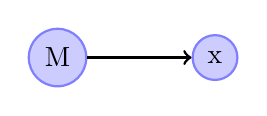
\begin{tikzpicture}[line width=1pt,  scale = 2]
\node[place] (M) at (0:0) {M};
\node[place] (x) at (0:1) {x};

\path[->] (M) edge (x);  
 \end{tikzpicture}
 \caption{Mother-child motif}
 \label{F:Mother-Child}
\end{figure}
Assume that mother node nourish the child node if the child is less than optimal, it won't nourish the child if it is at optimal or beyond. We set this optimal value for each component to be the same and set as $1$, which can be easily rescaled to any other value. We thus model this two-node network as following
\begin{equation}
\begin{array}{cc}
    \dot x_m  & = \alpha_m(1-\frac{x}{M}) - \beta \max(1-x, 0) x_m  \\
     \dot x = \alpha x(1-\frac{x}{})& 
\end{array}
\end{equation}



\section{Conclusion}
\section{Discussion}
\section*{Acknowledgements}




\printbibliography


\end{document}*************************************************

Key points:
\begin{enumerate}
\item Goal: understand the most profound principles of TCM. 
\item Why:
\begin{enumerate}
\item The greatest truths are the simplest. Examples in western culture: $F = ma$, $E = mc^2$.  
\item The TCM principles are accessible to average  people.
\item  TCM is effective  not only for minor health issue, but also for complex diseases such as cancers, and lupus. The many successful cases by a legendary Chinese Doctor Haisha Ni and his students are the great man  

\end{enumerate}
\item The Traditional Chinese Medicine
\end{enumerate}